\renewcommand{\arraystretch}{1.5}
\section{行列形式}
\ref{pi2flipper_sec}章で見たように共鳴条件を満たしたスピンフリッパーやシフタコイルの前後で波動関数の波数は変化しない。このことを利用すると波動関数から空間のつながりを切り離し、計算をエレガントに進めることができる。

\subsection{一般論}
\paragraph{行列形式とは}
この節では、一般にある領域の前後で波動関数の波数が変わらないとき、入射波と透過波で波動関数の空間成分は変化せず、時間・スピン成分はある空間に依存しない行列を介して変換されることを見る。

\begin{figure}[H]
\centering
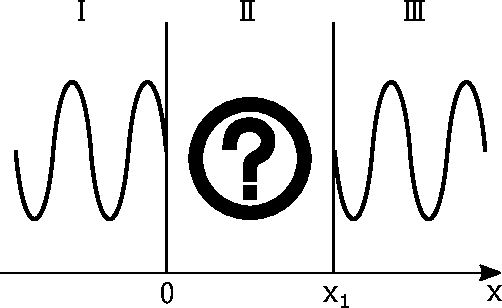
\includegraphics[height=3cm]{matrix/question.pdf}
\end{figure}
以下では簡単のために粒子のスピンを$1/2$とする。3つの領域I,II,IIIからなる系を考える。まず領域Iから波数$k$のスピン上向きの平面波
\begin{equation}
\psi^{\mathrm{inc}}=\begin{pmatrix} 1\\0 \end{pmatrix} \e^{ikx-i\omega_+ t}
\end{equation}
を入射する。Shr$\ddot{\mathrm{o}}$dinger方程式を系の境界条件のもとで解いて、領域IIIでの透過波が
\begin{equation}
\psi^{\mathrm{trans}}=\begin{pmatrix} a\e^{-i\omega_1t} \\ b\e^{-i\omega_2t} \end{pmatrix} \e^{ikx-i\omega_+ t}
\end{equation}
と求まったとする。ここで係数$a,b$やエネルギー変化$\omega_1,\omega_2$は入射波数と系の性質のみによってきまる定数とする。このときエネルギーは変わってもよいが、波数は変化していないことがポイントとなる。次に波数$k$のスピン下向き平面波
\begin{equation}
\psi^{\mathrm{inc}}=\begin{pmatrix} 0\\1 \end{pmatrix} \e^{ikx-i\omega_- t}
\end{equation}
を入射し、同様にShr$\ddot{\mathrm{o}}$dinger方程式を解いて領域IIIでの透過波が
\begin{equation}
\psi^{\mathrm{trans}}=\begin{pmatrix} c\e^{-i\omega_3t} \\ d\e^{-i\omega_4t} \end{pmatrix} \e^{ikx-i\omega_- t}
\end{equation}
と求まったとする。$c,d,\omega_3,\omega_4$も$a,b,\omega_1,\omega_2$と同様、入射波数と系の性質のみによってきまる定数とする。このときも波数は変化していない。すると、波数$k$の任意のスピン状態
\begin{equation}
\psi^{\mathrm{inc}}=\begin{pmatrix} p\e^{-i\omega_+t} \\ q\e^{-i\omega_-t}\end{pmatrix} \e^{ikx}
\end{equation}
を入射したときの領域IIIにおける透過波は、Shr$\ddot{\mathrm{o}}$dinger方程式の線形性から
\begin{equation}
\psi^{\mathrm{trans}}=\begin{pmatrix} a\e^{-i\omega_1t} & c\e^{-i\omega_3t} \\ b\e^{-i\omega_2t} & d\e^{-i\omega_4t} \end{pmatrix} \begin{pmatrix} p\e^{-i\omega_+t} \\ q\e^{-i\omega_-t}\end{pmatrix} \e^{ikx}
\end{equation}
となる。この結果は次のような見方ができる。すなわち波動関数を空間成分$K(x)$と時間・スピン成分$\chi(t)$に分けたとき、入射波と透過波で空間成分は変化せず
\begin{equation}
K^\mathrm{trans}(x)=K^\mathrm{inc}(x)=\e^{ikx}
\end{equation}
時間・スピン成分は変化しない入射波数と系の性質のみによって決まる行列$M(t)$を用いて
\begin{equation}
\chi^\mathrm{trans}(t)=M(t) \chi^\mathrm{inc}(t)
\end{equation}
と変換される。このような見方を行列形式と呼ぶことにする。上の例では
\begin{equation}
M(t)=\begin{pmatrix} a\e^{-i\omega_1t} & c\e^{-i\omega_3t} \\ b\e^{-i\omega_2t} & d\e^{-i\omega_4t} \end{pmatrix}
\end{equation}
である。ここで行列$M(t)$が時間のみに依存し、空間に依存しないことが重要な意味をもつ。

\paragraph{空間的な切り離し}
今度は7つの領域I,II,III,IV,V,VI,VIIからなる系を考える。ここで奇数番目の領域(I,III,V,VII)は全て同一の性質Oをもち、領域IIは性質Aを、領域IVは性質Bを、領域VIは性質Cをもつとする。さらに領域II、領域IV、領域VIの前後では波数が変化しないことが分かっている。
\begin{figure}[H]
\centering
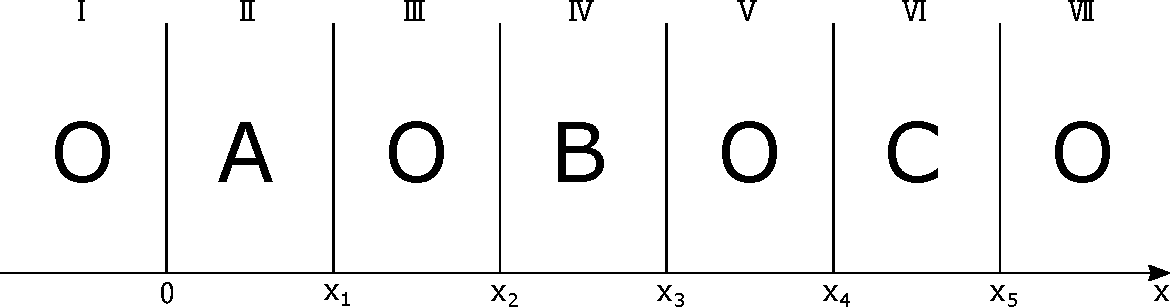
\includegraphics[height=3cm]{matrix/OABC.pdf}
\end{figure}
さて領域Iからスピン上向き平面波
\begin{equation}
\psi=\begin{pmatrix} 1\\0 \end{pmatrix} \e^{ik_+x-i\omega_0 t}
\end{equation}
を入射したとき領域VIIでの透過波はどのように表されるだろうか。もちろんShr$\ddot{\mathrm{o}}$dinger方程式を系の境界条件のもとで地道に解いてもよいが、ここでは前述の行列形式を用いよう。すなわち透過波を空間成分$K^\mathrm{trans}(x)$と時間・スピン成分$\chi^\mathrm{trans}(t)$に分け、性質A,B,Cから個別に求めた変換行列をそれぞれ$A(t),B(t),C(t)$とすると、
\begin{align}
&K^\mathrm{trans}=\e^{ik_+x} \\
&\chi^\mathrm{trans}=C(t)B(t)A(t) \begin{pmatrix} 1\\0 \end{pmatrix} \e^{-i\omega_0t}
\end{align}
と求まる。

ここで領域IIとIVの性質を入れ替える。つまり領域IIが性質Bを、領域IVが性質Aをもつとする。このとき先程と同様に領域Iからスピン上向き平面波を入射したときの領域VIIにおける透過波はどのように表されるか。Shr$\ddot{\mathrm{o}}$dinger方程式を解くとするとまた一から考える必要があるが、行列形式では変換行列が空間的な並びには依存しないことから
\begin{align}
&K^\mathrm{trans}=\e^{ik_+x} \\
&\chi^\mathrm{trans}=C(t)A(t)B(t) \begin{pmatrix} 1\\0 \end{pmatrix} \e^{-i\omega_0t}
\end{align}
とすぐに求まる。

このように行列形式の本質は領域の前後で波数が変わらないことを利用して、波動関数を空間的に形が変化しない空間成分と変化する時間・スピン成分に分けるところにある。それによって波動関数から空間的なつながりを切り離し、それぞれの領域を個別に考えた後で、好きな順番に並べ替えて議論することができる。

以下では具体的にそれぞれの装置の変換行列を求め、その後共鳴条件が満たされた場合のスピン干渉の式(\ref{})を再導出する。

\subsection{位相シフタコイル}
一様磁場中に位相シフタコイルがひとつ置かれた状況を考える。系は3つの領域I,II,IIIからなり、全体に$z$方向一様磁場$B_z$がかけられ、それに加えて領域IIに$z$方向一様磁場$B$がかけられている。
\begin{figure}[H]
\centering
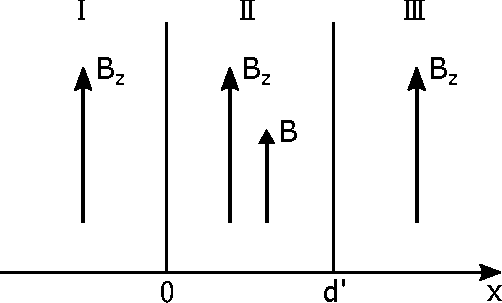
\includegraphics[height=3cm]{matrix/phaseshifter.pdf}
\end{figure}

\paragraph{領域I}
スピンの量子化軸を$z$軸に選ぶと、領域IにおけるShr$\ddot{\mathrm{o}}$dinger方程式は%なぜか\''{o}が使えない
\begin{equation}
i\frac{\del \psi_\mathrm{I}}{\del t}= \Biggl[-\frac{1}{2m} \frac{\del^2}{\del x^2} \underbrace{-\mu_nB_z}_{+|\mu_n|Bz =\omega_z} \sigma_z\Biggr] \psi_\mathrm{I}
\end{equation}
である。入射波数を$k$として、スピン上向き、下向きの入射波をそれぞれ
\begin{align}
\psi_\mathrm{I}=\begin{pmatrix} 1\\0 \end{pmatrix} \e^{i k x -i\omega_0 t} && \psi_\mathrm{I}=\begin{pmatrix} 0\\1 \end{pmatrix} \e^{i k x -i\omega^- t}
\end{align}
とすると
\begin{align}
&k=\sqrt{2m(\omega_0-\omega_z)} \\
&\omega^-=\frac{k^2}{2m} -\omega_z=\omega_0-2\omega_z
\end{align}
を得る。以後、入射エネルギーは外部磁場によるポテンシャルに比べて十分大きいとして近似し、全ての境界で反射を無視する。すなわち領域Iにおける波動関数は
\begin{align}
\psi_\mathrm{I}\simeq \begin{pmatrix} 1\\0 \end{pmatrix} \e^{i (k_0-\frac{\omega_z}{v}) x -i\omega_0 t} && \psi'_\mathrm{I}\simeq \begin{pmatrix} 0\\1 \end{pmatrix} \e^{i (k_0-\frac{\omega_z}{v}) x -i(\omega_0-2\omega_z) t}
\end{align}
と書ける。ここで$k_0 \equiv \sqrt{2m\omega_0},v \equiv k_0/m$とした。

\paragraph{領域II}
領域IIにおけるShr$\ddot{\mathrm{o}}$dinger方程式は
\begin{equation}
i\frac{\del \psi_\mathrm{II}}{\del t}= \left[-\frac{1}{2m} \frac{\del^2}{\del x^2} +(\omega_z+\omega) \sigma_z\right] \psi_\mathrm{II}
\end{equation}
ここで$\omega=|\mu_n|B$とした。領域IとIIの境界でエネルギーは変化しないので、領域IIにおけるスピン上下成分の波数$k^\pm_\mathrm{II}$は
\begin{align}
k^+_\mathrm{II}&=\sqrt{2m(\omega_0-(\omega_z+\omega))}\simeq k_0 -\frac{\omega_z}{v}-\frac{\omega}{v}\\
k^-_\mathrm{II}&=\sqrt{2m(\omega_0-2\omega_z+(\omega_z+\omega))}\simeq k_0 -\frac{\omega_z}{v}+\frac{\omega}{v}
\end{align}
となる。反射波を無視し、領域IとIIの境界(x=0)でそれぞれの入射波に対して波動関数を接続すると
\begin{align}
\psi_\mathrm{II}=\begin{pmatrix} 1\\0 \end{pmatrix} \e^{i (k_0-\frac{\omega_z}{v}-\frac{\omega}{v})x -i\omega_0 t} && \psi_\mathrm{II}=\begin{pmatrix} 0\\1 \end{pmatrix} \e^{i (k_0-\frac{\omega_z}{v} +\frac{\omega}{v}) x -i(\omega_0-2\omega_z) t}
\end{align}
を得る。

\paragraph{領域III}
領域IIIにおけるShr$\ddot{\mathrm{o}}$dinger方程式は領域Iと同じく
\begin{equation}
i\frac{\del \psi_\mathrm{I}}{\del t}= \Biggl[-\frac{1}{2m} \frac{\del^2}{\del x^2} +\omega_z \sigma_z\Biggr] \psi_\mathrm{I}
\end{equation}
である。領域IIとIIIの境界でエネルギーは変化しないので、領域IIIにおけるスピン上下成分の波数$k^\pm_\mathrm{III}$は
\begin{align}
k^+_\mathrm{III}=\sqrt{2m(\omega_0-\omega_z)}\simeq k_0 -\frac{\omega_z}{v}\\
k^-_\mathrm{III}=\sqrt{2m(\omega_0-2\omega_z+\omega_z)}\simeq k_0 -\frac{\omega_z}{v}
\end{align}
となる。領域IIとIIIの境界(x=d')でそれぞれの入射波に対して波動関数を接続すると
\begin{align}
\psi_\mathrm{III}=\begin{pmatrix} 1\\0 \end{pmatrix} \e^{-i\frac{\omega}{v}d'} \e^{i (k_0-\frac{\omega_z}{v})x -i\omega_0 t} && \psi_\mathrm{III}=\begin{pmatrix} 0\\1 \end{pmatrix} \e^{i\frac{\omega}{v}d} \e^{i (k_0-\frac{\omega_z}{v}) x -i(\omega_0-2\omega_z) t}
\end{align}
を得る。

\paragraph{変換行列}
以上より位相シフタコイルにおいて入射波と透過波の関係が次のように得られた:
\begin{align}
\psi_\mathrm{I}&= \begin{pmatrix} 1\\0 \end{pmatrix} \e^{i (k_0-\frac{\omega_z}{v}) x -i\omega_0 t} & \psi'_\mathrm{I}&= \begin{pmatrix} 0\\1 \end{pmatrix} \e^{i (k_0-\frac{\omega_z}{v}) x -i(\omega_0-2\omega_z) t} \\
\psi_\mathrm{III}&=\begin{pmatrix} 1\\0 \end{pmatrix} \e^{-i\frac{\omega}{v}d'} \e^{i (k_0-\frac{\omega_z}{v})x -i\omega_0 t} & \psi_\mathrm{III}&=\begin{pmatrix} 0\\1 \end{pmatrix} \e^{i\frac{\omega}{v}d} \e^{i (k_0-\frac{\omega_z}{v}) x -i(\omega_0-2\omega_z) t}
\end{align}
入射波と透過波を見比べることにより、位相シフタコイルの前後で波数は変化しないことが分かり、位相シフタコイルを表す変換行列$S$は
\begin{equation}
S=\begin{pmatrix} \e^{-i\frac{\omega}{v}d'} & 0\\0 &\e^{i\frac{\omega}{v}d'} \end{pmatrix}
\end{equation}
と求まる。

\subsection{共鳴スピンフリッパー}
一様磁場中に理想化されたRFスピンフリッパーがひとつ置かれた状況を考える。系は3つの領域I,II,IIIからなり、全体に$z$方向一様磁場$B_z$が、領域IIに$x$方向振動磁場$2B_r \cos \omega_s t$がかけられている。さらに以下では共鳴条件$\omega_s/2-\omega_z=0$が満たされている場合を扱う。
\begin{figure}[H]
\centering
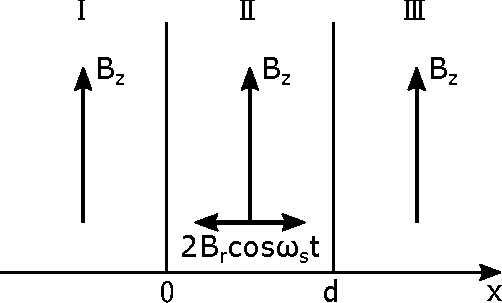
\includegraphics[height=3cm]{matrix/spinflipper.pdf}
\end{figure}

\paragraph{領域I}
領域Iは位相シフタコイルのときと全く同じで、波数$k$のスピン上向き、下向きの入射波はそれぞれ
\begin{align}
\psi_\mathrm{I}\simeq \begin{pmatrix} 1\\0 \end{pmatrix} \e^{i (k_0-\frac{\omega_z}{v}) x -i\omega_0 t} && \psi_\mathrm{I}\simeq \begin{pmatrix} 0\\1 \end{pmatrix} \e^{i (k_0-\frac{\omega_z}{v}) x -i(\omega_0-2\omega_z) t}
\end{align}
と表せる。

\paragraph{領域II}
\ref{pi2flipper_sec}章より領域IIにおける波動関数は反射波を無視すると一般に
\begin{equation}
\psi_\mathrm{II}=\begin{pmatrix} \left(A_n^+ \e^{ik_n^+x} -A_n^-\e^{ik_n^-x}\right)\e^{-i(\omega_n+\omega_z)} \\ \left(A_n^+ \e^{ik_n^+x} +A_n^-\e^{ik_n^-x} \right)\e^{-i(\omega_n-\omega_z)}\end{pmatrix}
\end{equation}
と書ける。ここで$k_n^\pm=\sqrt{2m(\omega_n\mp\omega_r)}$。よって$\psi_\mathrm{I}$と$\psi_\mathrm{II}$が領域IとIIの境界(x=0)において任意の時刻$t$で接続するためには
\begin{equation}
\omega_n=\omega_1\equiv \omega_0-\omega_z
\end{equation}
が必要である。そのとき
\begin{equation}
\psi_\mathrm{II}=\begin{pmatrix} \left(A_1^+ \e^{i(k_0-\frac{\omega_z}{v}-\frac{\omega_r}{v})x} -A_1^-\e^{i(k_0-\frac{\omega_z}{v}+\frac{\omega_r}{v})x}\right)\e^{-i\omega_0t} \\ \left(A_1^+ \e^{i(k_0-\frac{\omega_z}{v}-\frac{\omega_r}{v})x} +A_1^-\e^{i(k_0-\frac{\omega_z}{v}+\frac{\omega_r}{v})x}\right)\e^{-i(\omega_0-2\omega_z)t}\end{pmatrix}
\end{equation}
となる。領域IとIIの接続を考えると、スピン上向き、下向きの入射波に対してそれぞれ
\begin{align}
&\begin{cases}A_1^+-A_1^-=1\\A_1^++A_1^-=0\end{cases} &&\begin{cases}A_1^++A_1^-=1\\A_1^+-A_1^-=0\end{cases} \notag \\
&\Rightarrow \begin{cases} A_1^+=\frac{1}{2} \\ A_1^-=-\frac{1}{2}\end{cases} &&\Rightarrow \begin{cases} A_1^+=\frac{1}{2} \\ A_1^-=\frac{1}{2}\end{cases}
\end{align}
がなりたつ。したがってそれぞれの入射波に対する領域IIの波動関数は
\begin{align}
\psi_\mathrm{II} &=\begin{pmatrix} \frac{1}{2} \left(\e^{i(k_0-\frac{\omega_z}{v}-\frac{\omega_r}{v})x}+\e^{i(k_0-\frac{\omega_z}{v}+\frac{\omega_r}{v})x}\right) \e^{-i\omega_0t} \\ \frac{1}{2} \left(\e^{i(k_0-\frac{\omega_z}{v}-\frac{\omega_r}{v})x}-\e^{i(k_0-\frac{\omega_z}{v}+\frac{\omega_r}{v}x}\right) \e^{-i(\omega_0-2\omega_z)t}\end{pmatrix} &\psi_\mathrm{II}&=\begin{pmatrix} \frac{1}{2} \left(\e^{i(k_0-\frac{\omega_z}{v}-\frac{\omega_r}{v})x}-\e^{i(k_0-\frac{\omega_z}{v}+\frac{\omega_r}{v})x}\right) \e^{-i\omega_0t} \\ \frac{1}{2} \left(\e^{i(k_0-\frac{\omega_z}{v}-\frac{\omega_r}{v})x}+\e^{i(k_0-\frac{\omega_z}{v}+\frac{\omega_r}{v}x}\right) \e^{-i(\omega_0-2\omega_z)t}\end{pmatrix} \notag \\
&=\begin{pmatrix} \cos \frac{\omega_r x}{v} \e^{i(k_0-\frac{\omega_z}{v})x}\e^{-\omega_0t} \\ -i\sin\frac{\omega_r x}{v} \e^{i(k_0-\frac{\omega_z}{v})x}\e^{-i(\omega_0-2\omega_z)t} \end{pmatrix} &&=\begin{pmatrix} -i\sin\frac{\omega_rx}{v} \e^{i(k_0-\frac{\omega_z}{v})x}\e^{-\omega_0t} \\ \cos \frac{\omega_r x}{v} \e^{i(k_0-\frac{\omega_z}{v})x}\e^{-i(\omega_0-2\omega_z)t} \end{pmatrix}
\end{align}
となる。

\paragraph{領域III}
領域IIIも位相シフタコイルのときと同様にして、領域IIIにおけるスピン上下成分の波数$k^\pm_\mathrm{III}$は
\begin{align}
k^+_\mathrm{III}=\sqrt{2m(\omega_0-\omega_z)}\simeq k_0 -\frac{\omega_z}{v}\\
k^-_\mathrm{III}=\sqrt{2m(\omega_0-2\omega_z+\omega_z)}\simeq k_0 -\frac{\omega_z}{v}
\end{align}
となる。領域IIとIIIの境界(x=d)でそれぞれの入射波に対して波動関数を接続すると
\begin{align}
\psi_\mathrm{III}=\begin{pmatrix} \cos \frac{\omega_r d}{v} \e^{i(k_0-\frac{\omega_z}{v})x}\e^{-\omega_0t} \\ -i\sin\frac{\omega_r d}{v} \e^{i(k_0-\frac{\omega_z}{v})x}\e^{-i(\omega_0-2\omega_z)t} \end{pmatrix} &&\psi_\mathrm{III}=\begin{pmatrix} -i\sin\frac{\omega_rd}{v} \e^{i(k_0-\frac{\omega_z}{v})x}\e^{-\omega_0t} \\ \cos \frac{\omega_r x}{v} \e^{i(k_0-\frac{\omega_z}{v})d}\e^{-i(\omega_0-2\omega_z)t} \end{pmatrix}
\end{align}
を得る。

\paragraph{変換行列}
以上より共鳴条件を満たしたスピンフリッパーにおいて入射波と透過波の関係が次のように得られた:
\begin{align}
\psi_\mathrm{I}&= \begin{pmatrix} 1\\0 \end{pmatrix} \e^{i (k_0-\frac{\omega_z}{v}) x -i\omega_0 t} &\psi_\mathrm{I}&= \begin{pmatrix} 0\\1 \end{pmatrix} \e^{i (k_0-\frac{\omega_z}{v}) x -i(\omega_0-2\omega_z) t}\\
\psi_\mathrm{III}&=\begin{pmatrix} \cos \frac{\omega_r d}{v} \e^{i(k_0-\frac{\omega_z}{v})x}\e^{-\omega_0t} \\ -i\sin\frac{\omega_r d}{v} \e^{i(k_0-\frac{\omega_z}{v})x}\e^{-i(\omega_0-2\omega_z)t} \end{pmatrix} &\psi_\mathrm{III}&=\begin{pmatrix} -i\sin\frac{\omega_rd}{v} \e^{i(k_0-\frac{\omega_z}{v})x}\e^{-\omega_0t} \\ \cos \frac{\omega_r d}{v} \e^{i(k_0-\frac{\omega_z}{v})x}\e^{-i(\omega_0-2\omega_z)t} \end{pmatrix}
\end{align}
入射波と透過波を見比べることにより、共鳴スピンフリッパーの前後で波数は変化しないことが分かり、共鳴スピンフリッパーを表す変換行列$F$は
\begin{equation}
F=\begin{pmatrix} \cos \frac{\omega_r d}{v} &-i\sin\frac{\omega_rd}{v}\e^{-2i\omega_zt} \\ -i\sin\frac{\omega_rd}{v}\e^{+2i\omega_zt} &\cos \frac{\omega_r d}{v}\end{pmatrix}
\end{equation}
と求まる。

\subsection{スピン干渉}
いよいよ行列形式でスピン干渉を見てゆく。一様磁場中にスピンフリッパー、位相シフタコイル、スピンフリッパーが順番に置かれた状況を考える。系は7つの領域I,II,III,IV,V,VI,VIIからなり、全体に$z$方向一様磁場$B_z$がかけられ、それに加えて領域II,VIに$x$方向振動磁場$2B_r\cos\omega_s t$が、領域IVに$z$方向一様磁場$B$がかけられている。
\begin{figure}[H]
\centering
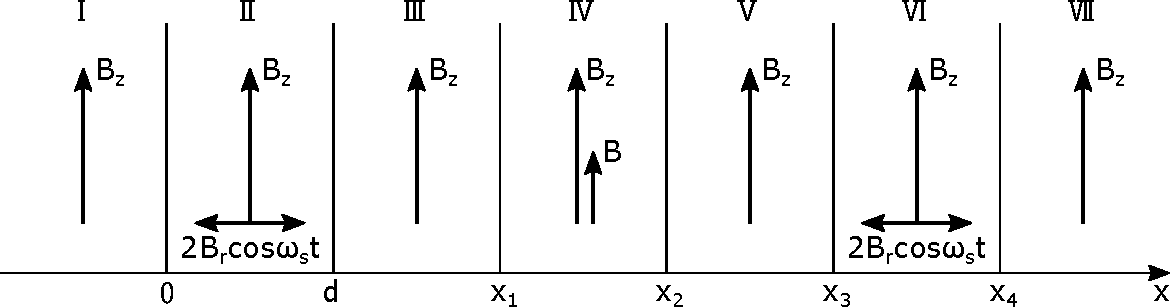
\includegraphics[height=3cm]{matrix/interference.pdf}
\end{figure}

領域Iからスピン上向き平面波
\begin{equation}
\psi_\mathrm{I}(x,t)=\underbrace{\begin{pmatrix} 1\\0\end{pmatrix} \e^{-i\omega_0t}}_{\chi_\mathrm{I}(t)} \underbrace{\e^{i (k_0-\frac{\omega_z}{v})x}}_{K_\mathrm{I}(x)}
\end{equation}
を入射したとき、領域VIIにおける波動関数$\psi_\mathrm{VII}(x,t)$の空間成分$K_\mathrm{VII}(x)$と時間・スピン成分$\chi_\mathrm{VII}(t)$は
\begin{align}
K_\mathrm{VII}(x)=K_\mathrm{I}(x)=\e^{i (k_0-\frac{\omega_z}{v})x}
\end{align}
\begin{align}
\chi_\mathrm{VII}(t)&=FSF\chi_\mathrm{I}(t) \notag \\
&=\scalebox{0.9}{$\begin{pmatrix} \cos \frac{\omega_r d}{v} &-i\sin\frac{\omega_rd}{v}\e^{-2i\omega_zt} \\ -i\sin\frac{\omega_rd}{v}\e^{+2i\omega_zt} &\cos \frac{\omega_r d}{v}\end{pmatrix}\begin{pmatrix} \e^{-i\frac{\omega}{v}d'} & 0\\0 &\e^{i\frac{\omega}{v}d'} \end{pmatrix}\begin{pmatrix} \cos \frac{\omega_r d}{v} &-i\sin\frac{\omega_rd}{v}\e^{-2i\omega_zt} \\ -i\sin\frac{\omega_rd}{v}\e^{+2i\omega_zt} &\cos \frac{\omega_r d}{v}\end{pmatrix} \begin{pmatrix} 1\\0\end{pmatrix} \e^{-i\omega_0t}$} \notag \\
&=\begin{pmatrix} \cos^2 \frac{\omega_r d}{v} \e^{-i\frac{\omega d'}{v}} -\sin^2 \frac{\omega_r d}{v} \e^{i\frac{\omega d'}{v}} \\ -i\sin\frac{\omega_r d}{v}\cos\frac{\omega_r d}{v}\left(\e^{-i\frac{\omega d'}{v}}+\e^{i\frac{\omega d'}{v}} \right) \e^{i\omega_s t} \end{pmatrix}\e^{-i\omega_0t}
\end{align}
となる。したがって領域VIIにおいてスピン上向き中性子を観測する確率は
\begin{align}
|\psi_\mathrm{VII}^+|^2&=|\chi_\mathrm{VII}^+|^2=\Biggl|\cos^2 \frac{\omega_r d}{v} \e^{-i\frac{\omega d'}{v}} -\sin^2 \frac{\omega_r d}{v} \e^{i\frac{\omega d'}{v}}\Biggr|^2\notag \\
&=\cos^4 \frac{\omega_r d}{v} +\sin^4 \frac{\omega_r d'}{v} -2\sin^2\frac{\omega_rd}{v}\cos^2\frac{\omega_rd}{v} \cos \frac{2\omega d'}{v} \notag \\
&=1-\sin^2 \frac{2\omega_r d}{v} \cos^2 \frac{\omega d'}{v}
\end{align}
となる。確かに\ref{pi2flipper_sec}章で得られた結果が再び得られた。
\renewcommand{\arraystretch}{1}





